\documentclass[border=6pt]{standalone}
\usepackage[T1]{fontenc}
\usepackage{lmodern}\usepackage{tgtermes}
\usepackage{amsmath,amssymb,xcolor,tikz}
\usetikzlibrary{arrows.meta,calc,positioning}
\tikzset{
  bus/.style={line width=2.4pt},
  ln/.style={line width=0.8pt},
  gen/.style={circle, draw, line width=0.8pt, minimum size=9mm, inner sep=0pt, font=\small},
  load/.style={-{Stealth[length=2.6mm]}, line width=0.8pt},
  lab/.style={font=\footnotesize, fill=white, inner sep=1.5pt},
  res/.style={font=\footnotesize\bfseries, inner sep=1pt},
}


\begin{document}
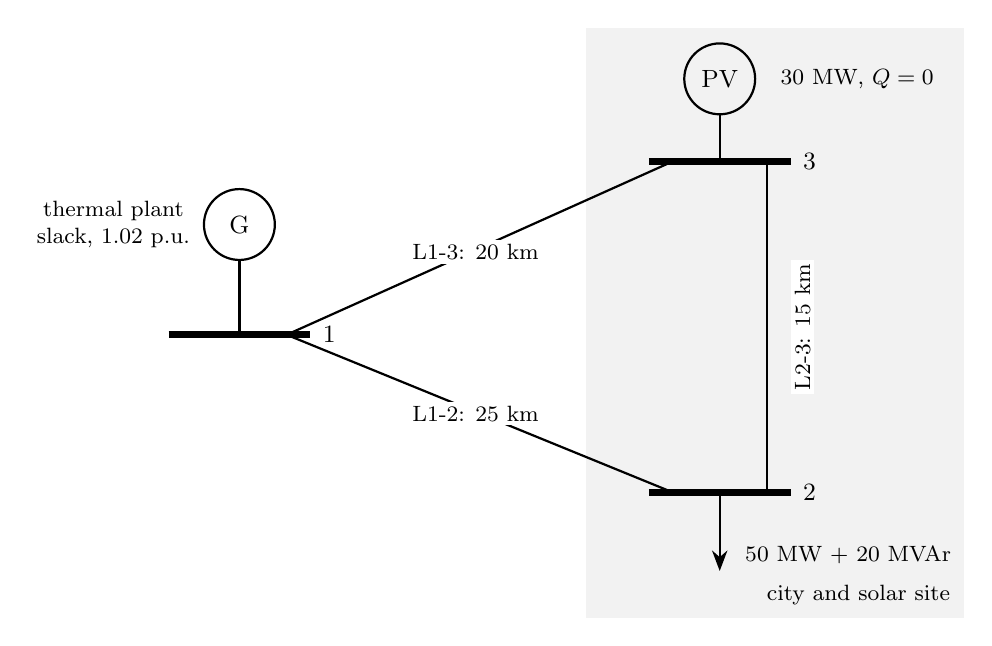
\begin{tikzpicture}
  \fill[gray!10] (4.4,-3.6) rectangle (9.2,3.9);
  \node[font=\footnotesize, anchor=south east] at (9.15,-3.55) {city and solar site};
  \draw[bus] (-0.9,0) -- (0.9,0) node[right, font=\small] {1};
  \draw[bus] (5.2,2.2) -- (7.0,2.2) node[right, font=\small] {3};
  \draw[bus] (5.2,-2.0) -- (7.0,-2.0) node[right, font=\small] {2};
  \node[gen] (g) at (0,1.4) {G}; \draw[ln] (g) -- (0,0);
  \node[font=\footnotesize, align=center] at (-1.6,1.4) {thermal plant\\slack, 1.02 p.u.};
  \node[gen] (pv) at (6.1,3.25) {PV}; \draw[ln] (pv) -- (6.1,2.2);
  \node[font=\footnotesize, align=left, anchor=west] at (6.75,3.25) {30 MW, $Q = 0$};
  \draw[load] (6.1,-2.0) -- (6.1,-3.0); \node[font=\footnotesize, anchor=west] at (6.3,-2.8) {50 MW + 20 MVAr};
  \draw[ln] (0.6,0) -- (5.5,2.2); \draw[ln] (0.6,0) -- (5.5,-2.0); \draw[ln] (6.7,-2.0) -- (6.7,2.2);
  \node[lab] at (3.0,1.05) {L1-3: 20 km};
  \node[lab] at (3.0,-1.0) {L1-2: 25 km};
  \node[lab, rotate=90] at (7.15,0.1) {L2-3: 15 km};
\end{tikzpicture}
\end{document}
